\section{The Problem}
Now that we have determined a sensible illumination normalization technique to use, we turn our 
attention to another means of improving recognition rates.  When we consider the problem we are
trying to solve, namely facial recognition for classroom attendance tracking, we realise that 
the current method of classification used by the Eigenface method doesn't make any use of the 
intrinsic properties of our problem. \\

We know exactly who and how many subjects should present in each lecture.  Knowing this, we can 
in theory improve our recognition rates by doing away with Eigenfaces current greedy, first match 
algorithm and in its place use a global assignment algorithm like the Hungarian Algorithm which 
we shall look into in the following sections. \\

The following chapter discusses but does not implement the following features due to constraints 
that are discussed at the end of the chapter.  In its current state the provided Eigenface 
algorithm makes use of a greedy first match algorithm.  When you don't know the sets you are dealing 
with and whether or not the face you are testing is even in your data set, it is a adequate solution.  
It will take a test face and try find the best match it can in its training data as well as providing 
a matching confidence.  \\
	
However, we do know the sets, and are sufficiently confident that every face we test is in our training 
data.  Thus we can surely use this knowledge by making use of a multiple assignment optimisation 
algorithm.  Such an algorithm scores every test face against all training faces, thereafter, optimise 
the classification of who's who to minimize the total score of the entire classification.

\section{The Assignment problem}
The assignment problem details the complexity of assigning two sets to one another such that some cost 
is minimised.  Doing so has many real world applications; Logistics of Assigning cargo to ships/trucks 
to minimise fuel costs based on their varying shipping/land routes~\cite{Assignmentproblems}, assigning 
jobs to various employees to yield the least possible wage expense etc. 

  	\begin{figure}[H]
		\centering
		\caption{The Assignment problem \label{fig:Assign_part1}}
		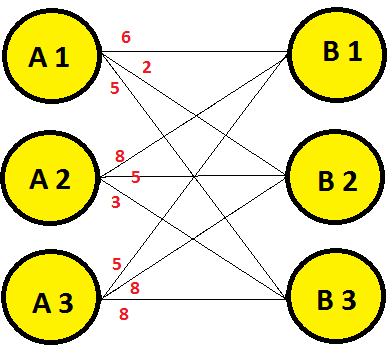
\includegraphics[width=95mm,height=95mm]{Assign_part1.png}
	\end{figure}
	
Above in fig:[~\ref{fig:Assign_part1}] details a problem of assigning set A to B we see that each 
connection has an associated cost involved.  We note each branch varies in cost thus mathematically, 
different selections would have different costs incurred, hence there must exist one selection that 
has a cost less than or equal to all other combinations. 

  	\begin{figure}[H]
		\centering
		\caption{The Assignment problem solution \label{fig:Assign_part2}}
		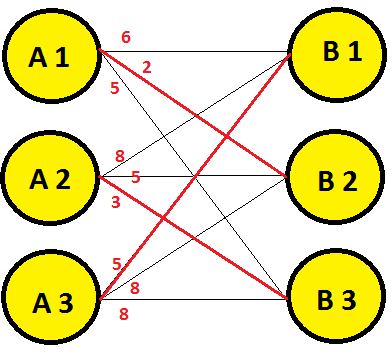
\includegraphics[width=95mm,height=95mm]{Assign_part2.png}
	\end{figure}

We see from fig:[~\ref{fig:Assign_part2}] that the cheapest matching is the selection [A1,B2],[A2,B3],
[A3,B1] now doing this by eye was trivial enough for these sets.  Now what if we had 100 elements per 
set?  Clearly what we need to do is find an algorithm that can solve this problem for us within a 
reasonable time.  To this end, we look at the Hungarian Algorithm~\cite{Hungarian_alg}.
 
\section{Hungarian Algorithm}
The Hungarian Algorithm is a proposed solution to the assignment problem that is solved by minimizing the 
total costs of all assignments.  Since Eigenface matching measures the difference between the feature 
vector of a probe face compared to the feature vectors of the training faces, a close match returns a low 
number.  So for our problem, we wish to minimise the overall difference.  As we work with a matching score that 
is better the smaller it is, we have a classic minimisation problem to which the Hungarian Algorithm is well 
suited. \\

In order for the algorithm to work it needs to be able to build up a square matrix i.e. the two sets you 
wish to match must be of the same length.  With this in place we would score the data, putting the 
confidences attained in an output matrix $m_{n \times n}$.  The element $m_{i \times j}$ where $i,j < n$ 
of the this matrix would then indicate the Eigenface score of probe feature vector $i$ against the feature 
vector of the training face $j$.  Now the problem involves choosing a combination of scores such that the 
total combination of these scores is as small as possible. \\

One point we need to take into account is the situation where we have less students present than there 
should be or the less likely situation where there are more.  These are concerns because as previously stated, 
the Hungarian Algorithm needs a square matrix to operate on.  We have two options: we can pad with high numbers 
or zeros.  Standard procedure is to pad the rows or columns with values equal to the highest present value 
currently in the matrix.  Thus those present get the best chance at matching the faces in the set i.e. the 
assignment of subject $n$ to training subject three with a confidence of 300 isn't stolen by one of our made up 
padded students who we gave a stronger match by setting the padding to 0. \\

We could do this by hand for small sets, but the problem quickly escalates as the sets become bigger 
in fact the problem done this way is of O(n!) not ideal.  However at the core of the Hungarian Algorithm 
is the theorem: If a number is added to or subtracted from all of the entries of any one row or column 
of a cost matrix, then an optimal assignment for the resulting cost matrix is also an optimal assignment 
for the original cost matrix ~\cite{Hungarian_alg}. This observation allows us to force the least cost 
in a row or column to be represented as a zero.  In turn, this provides an efficient way of ``eliminating'' 
rows and columns from the matrix to reduce the size of the remaining problem. \\

The algorithm from ~\cite{Hungarian_alg};
\begin{enumerate}
	\item Firstly, subtract the smallest entry in each row from all the other entries in that row.  Now do the same for each column. 
	\item Select rows and columns so that all zero elements are selected with the minimum number of selections. 
	\item (I) If the number of selections is n, then we are done, we have found the optimal assignment. \\
		  (II) If we have less than n selections an optimal selection is not yet possible, so we proceed. 
	\item Determine smallest entry not yet covered by any line, subtract this value from each element in every unselected row 
		  and add it to each element in each selected column.   Return to step 2.
\end{enumerate}

Below is a working example of the Hungarian Algorithm, given fig:[~\ref{fig:select_step_1}]
  	
	\begin{figure}[H]
		\centering
		\caption{Initial matrix \label{fig:select_step_1}}
		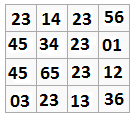
\includegraphics[width=50mm,height=50mm]{select_step_1_Hungarian.png}
	\end{figure}
	
Performing the first step (least value row subtraction) we get fig:[~\ref{fig:select_step_1_1}]

	\begin{figure}[H]
		\centering
		\caption{Subtraction of least value per row \label{fig:select_step_1_1}}
		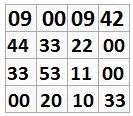
\includegraphics[width=50mm,height=50mm]{select_step_1_1_Hungarian.png}
	\end{figure}

Performing the second step (least value column subtraction) we then get fig:[~\ref{fig:select_step_2}]

  	\begin{figure}[H]
		\centering
		\caption{Subtraction of least value per column \label{fig:select_step_2}}
		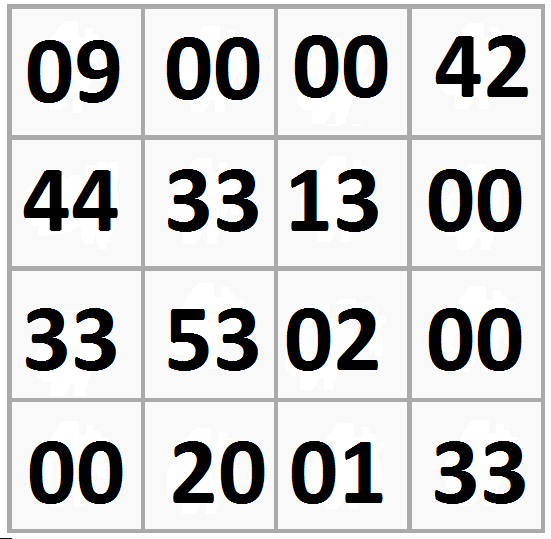
\includegraphics[width=50mm,height=50mm]{select_step_2_Hungarian.png}
	\end{figure}
	

So, mathematically, we can manipulate along rows or down columns by the same operation without it affecting
the integrity of the matrix.  We know this thanks to the afore mentioned theorem the proof of which is 
beyond the scope of this work.  However, we have another aspect to look at, how exactly do we find the 
minimum selection of rows/columns that contain all our zeroed elements? One way this can be done is as 
follows; \\

\begin{itemize}	
 \item First as seen in fig:[~\ref{fig:select_step_3}], make as many minimum cost assignments as possible 
 without double assigning.  In the provided example we have designated this with an apostrophe.  We select 
 [4,1] as an option as it has no conflicts.  However, for row 1 we need to make a choice, this choice can 
 safely be made arbitrarily.  Doing so we select [1,2] instead of [1,3] similarly we must choose between 
 [2,4] and [3,4] we choose [2,4].
\end{itemize}

  	\begin{figure}[H]
		\centering
		\caption{Selection of rows and columns step 1 \label{fig:select_step_3}}
		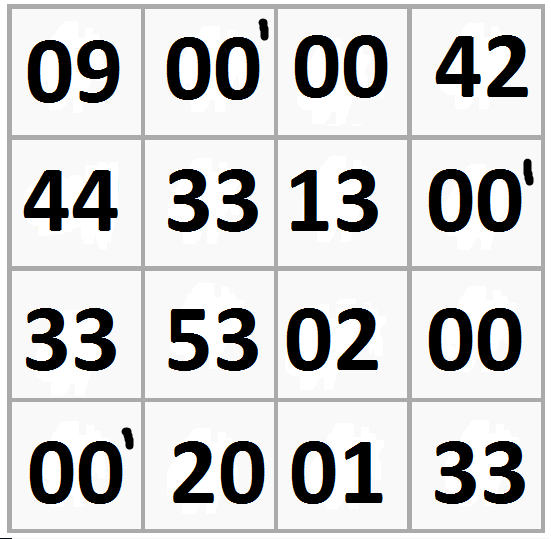
\includegraphics[width=50mm,height=50mm]{select_step_3_Hungarian.png}
	\end{figure}

\newpage	
Step 2:
\begin{itemize}
 \item Now, mark all rows having no assignments (zeros marked with apostrophes) (row 3) Shown as (X1) in the following diagram
 \item Next, mark all unmarked columns having zeros in newly marked rows (column 4) (X2)
 \item mark all rows having assignments in newly marked columns (row 2) (X3)
\end{itemize}

Doing the above we end up with fig:[~\ref{fig:select_step_4}] 

  	\begin{figure}[H]
		\centering
		\caption{Selection of rows and columns step 2 \label{fig:select_step_4}}
		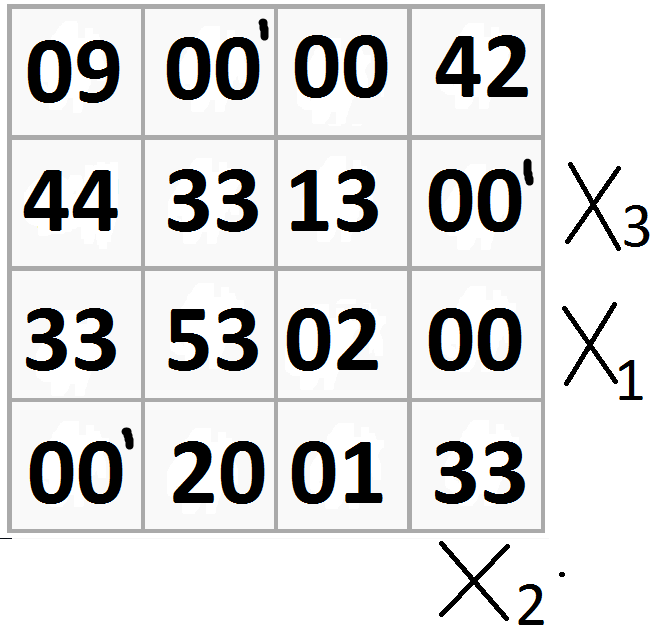
\includegraphics[width=50mm,height=50mm]{select_step_4_Hungarian.png}
	\end{figure}

\begin{itemize}	
 \item Finally make your selections on all marked columns and all UNMARKED rows.  
\end{itemize}

  	\begin{figure}[H]
		\centering
		\caption{Selection of rows and columns step 3 \label{fig:select_step_5}}
		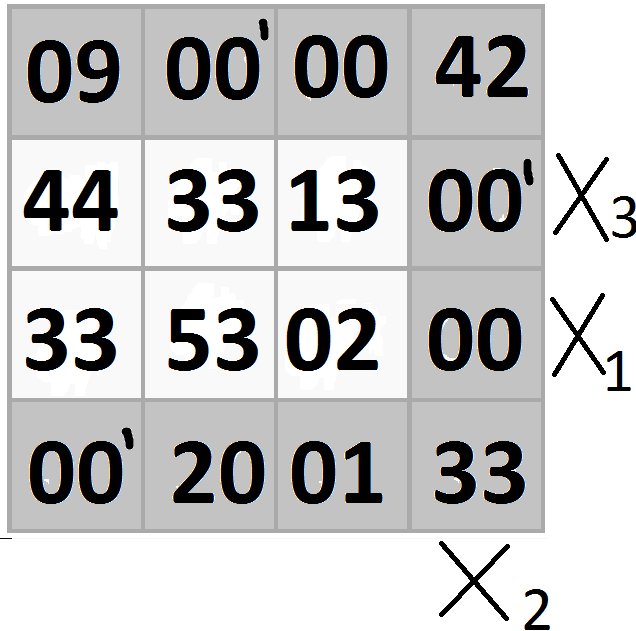
\includegraphics[width=50mm,height=50mm]{select_step_5_Hungarian.png}
	\end{figure}
	
We now end up with the minimum row and column selections we would need to make to select all zeros 
in the graph.  With this we can determine if we are done.  We count our selection lines totalling 
three, as this is less than our set size we move on to step four of the Hungarian Algorithm.  Doing 
this we get fig:[~\ref{fig:select_step_6}] 
	
  	\begin{figure}[H]
		\centering
		\caption{Final State.\label{fig:select_step_6}}
		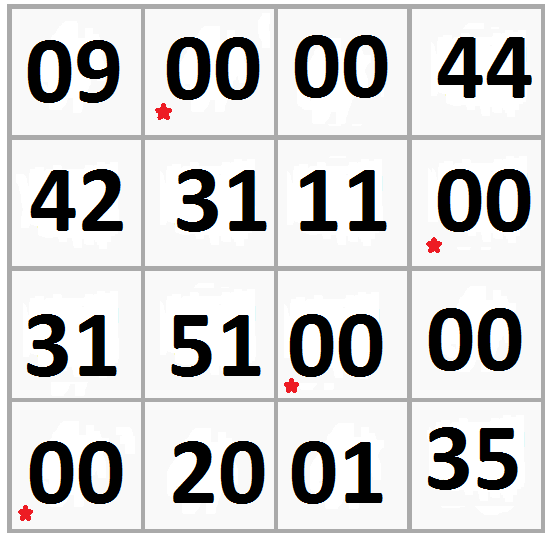
\includegraphics[width=50mm,height=50mm]{select_step_6_Hungarian.png}
	\end{figure}

Now, if necessary, one would rinse and repeat from step 3 to get the minimum cost assignment.  However 
for this example we are now done and get the minimum cost assignment of (row, col)[4,1][1,2][2,4][3,3] 
which going back to fig:[~\ref{fig:select_step_1}] gives a total cost of: 41.  \\

The above is just one way of making the minimum number of selections.  The method was learned from 
wikepedia.

\section{Summary}
This chapter looked into the possibility of using a global optimisation technique for assignment of 
two sets.  We predict that doing so will improve accuracy of the recognition software used by the system.  
We focused on the Hungarian Algorithm as the solution we would implement.  Detailing the steps needed to make it 
work, also noting that eigenfaces method of scoring lends itself nicely to such a minimising solution. \\

Sadly, we cannot in a simple manner implement such a system, as we cannot easily force the Eigenface method to 
provide all the scores of the test data against all training vectors.  There are some hints around the Internet 
as to how to achieve what we wish to do.  For example~\cite{Eigenface_classification} shows us that we could 
extend the \texttt{predict} function to provide us with an array containing the distances scored for each 
training component.  However, it would require diving into OpenCV and extending the existing functionality 
and also could become obsolete if a future superior implementation of the algorithm is designed.  \\

Regardless, time did not permit such alterations to be made within the scope of this work.  Hence this change 
is proposed as possible future work at least until OpenCV provides such functionality itself as was hinted at 
in~\cite{Eigenface_classification}. \\

